\documentclass[11pt,a4paper]{article}

\usepackage[utf8]{inputenc}
\usepackage[T1]{fontenc}
\usepackage[english]{babel}
\usepackage{lmodern}
\usepackage{amsmath,amssymb}
\usepackage{graphicx}
\usepackage{booktabs}
\usepackage{microtype}
\usepackage{xcolor}
\usepackage{hyperref}
\usepackage{geometry}
\usepackage{caption}
\usepackage{float}
\usepackage{siunitx}
\usepackage[most]{tcolorbox}

\geometry{margin=2.4cm}
\graphicspath{{figures/}}
\hypersetup{colorlinks=true,linkcolor=blue!60!black,citecolor=blue!60!black,urlcolor=blue!60!black}
\sisetup{range-phrase=--,range-units=single}

% Highlight boxes for central results
\newtcolorbox{merke}{colback=blue!5!white,colframe=blue!50!black,title=Key point,fonttitle=\bfseries}
\newtcolorbox{rechnung}{colback=gray!8!white,colframe=gray!60!black,title=Step by step,fonttitle=\bfseries,breakable}

\newcommand{\VDD}{V_{DD}}
\newcommand{\VT}{V_{T}}
\newcommand{\ovl}[1]{\overline{#1}}

\title{\textbf{A Look-Up Table Built from Transistors}\\[0.3em]
\large How twenty MOSFETs and four stored bits become any logic function
of two inputs -- the logic element of an FPGA, derived, drawn and simulated}
\author{Stephan Bökelmann}
\date{}

\begin{document}
\maketitle
\thispagestyle{empty}

\begin{abstract}
\noindent
How can one and the same circuit be an AND gate today and an XOR gate
tomorrow, without a single wire being moved? This is the question behind
every field-programmable gate array (FPGA), and the answer is the
look-up table (LUT). This text builds a LUT with two inputs from the
ground up in six steps: (1)~A logic function of $k$ inputs is nothing but
its truth table, a list of $2^k$ bits; there are 16 such functions for
$k=2$. (2)~A circuit that \emph{stores} these bits and \emph{selects}
one of them with its inputs therefore realises every function, and the
selection is a tree of 2:1 multiplexers -- Shannon's expansion theorem
drawn as hardware. (3)~A multiplexer is two switches, and a switch is a
MOS transistor; we compute from the transistor model why a single NMOS
hands over a~1 only up to \SI{3.5}{V} and why an NMOS and a PMOS in
parallel, the transmission gate, hand over both levels in full.
(4)~A CMOS inverter restores the logic level; we compute its switching
threshold and the current it draws. (5)~The complete circuit has 20
transistors; its four stored bits are the \emph{configuration}, and here
they are voltage sources, so that the function of the LUT can be read
off the schematic. (6)~A transient simulation with ngspice steps through
all 16 functions in one run and measures delays, levels and the
behaviour when both inputs change at once. All calculations are carried
out explicitly, every number in the text is reproduced by the code in the
accompanying repository, and the primary sources are cited throughout.
The only prerequisites are Boolean algebra at school level and the idea
of a transistor as a voltage-controlled switch.
\end{abstract}

\tableofcontents
\vspace{1em}

% ============================================================
\section{Introduction: the common thread}
% ============================================================

A logic gate is a circuit that computes a fixed Boolean function. An AND
gate made from transistors will be an AND gate for the rest of its life;
the function is wired in. A \emph{programmable} logic device must be
different in kind: it has to be able to become an AND gate, an OR gate,
or an XOR gate after it has been manufactured, by writing a few bits into
it, and it must be able to forget and become something else. Every
field-programmable gate array (FPGA) contains tens of thousands to
millions of such elements, and in nearly all of them the element is the
same: a \textbf{look-up table}, or LUT.

The idea of the look-up table is older than the transistor. A table of
logarithms does not compute a logarithm; it stores the answers to all
questions one is likely to ask and lets the reader select the right row.
A LUT does the same with a Boolean function. It does not compute
anything. It stores the \emph{truth table} of the function, one bit per
row, and uses its inputs to select which of these bits appears at the
output. Which function it realises is decided by what is stored, not by
how it is built. That is what makes it programmable.

This text follows this idea down to the transistor and back up to the
simulation, in one continuous line of reasoning:

\begin{enumerate}
    \item A Boolean function \emph{is} its truth table
          (Section~\ref{sec:functions}). For two inputs there are four
          rows and therefore $2^4=16$ functions.
    \item Selecting one of four stored bits by two inputs is a tree of
          2:1 multiplexers (Section~\ref{sec:mux}). Shannon's expansion
          theorem says that this tree is not one possible structure for a
          LUT but \emph{the} structure.
    \item A 2:1 multiplexer is two switches, and a switch is a MOS
          transistor (Section~\ref{sec:switch}). The transistor model
          tells us that one transistor is not enough, and why two in
          parallel are.
    \item The output of the multiplexer tree must be restored and
          buffered; this is the job of two CMOS inverters
          (Section~\ref{sec:inverter}).
    \item Put together, the circuit has 20 transistors
          (Section~\ref{sec:circuit}). Its four stored bits are the
          configuration; in this text they are voltage sources, in an
          FPGA they are memory cells written by the bitstream.
    \item A simulation of the complete transistor circuit confirms that
          it computes all 16 functions, and measures how fast
          (Section~\ref{sec:simulation}).
\end{enumerate}

Everything in this text can be reproduced. The circuit is described in
Python with SKiDL, written as a hierarchical KiCad schematic, simulated
with ngspice, and viewed in GTKWave; the repository
\url{https://github.com/MaxClerkwell/transistor-lut} contains the code,
the schematic, the results and the scripts that produced every figure
of this text.

% ============================================================
\section{A Boolean function is its truth table}
\label{sec:functions}
% ============================================================

\subsection{Functions of two inputs}

Let $A$ and $B$ be two logic variables, each either 0 or 1. A Boolean
function $f(A,B)$ assigns to each of the four possible input
combinations $(A,B)\in\{00,10,01,11\}$ an output value 0 or~1. Boole
introduced this algebra of two values in 1854 as a calculus of
propositions~\cite{Boole1854}; Shannon showed in 1938 that it describes
switching circuits exactly~\cite{Shannon1938}, and from then on a
Boolean function and a circuit built from switches have been two views
of the same thing.

The complete description of $f$ is its \textbf{truth table}: four rows,
one output bit each. Nothing else about $f$ exists. Whether we write
$f=A\cdot B$ or $f=\ovl{\ovl{A}+\ovl{B}}$ makes no difference to the
table, and two expressions with the same table are the same function.

\subsection{How many functions are there?}

A function of $k$ inputs has a truth table of $2^k$ rows. Each row holds
one bit, which can be chosen independently of all the others, so the
number of distinct functions is
\begin{equation}
    N_k = 2^{\,2^k}.
    \label{eq:count}
\end{equation}
For $k=2$ this is $2^4=16$; for $k=4$ it is $2^{16}=65\,536$; for $k=6$
it is $2^{64}\approx1.8\times10^{19}$. The 16 functions of two inputs
are shown in Figure~\ref{fig:truth_tables}, each as a column of four
bits. Among them are all the familiar gates: AND, OR, NAND, NOR, XOR,
XNOR, the two inverters $\ovl A$ and $\ovl B$, the two wires $A$ and
$B$, the constants 0 and 1, and four less familiar ones such as
$A\cdot\ovl B$.

\begin{figure}[H]
\centering
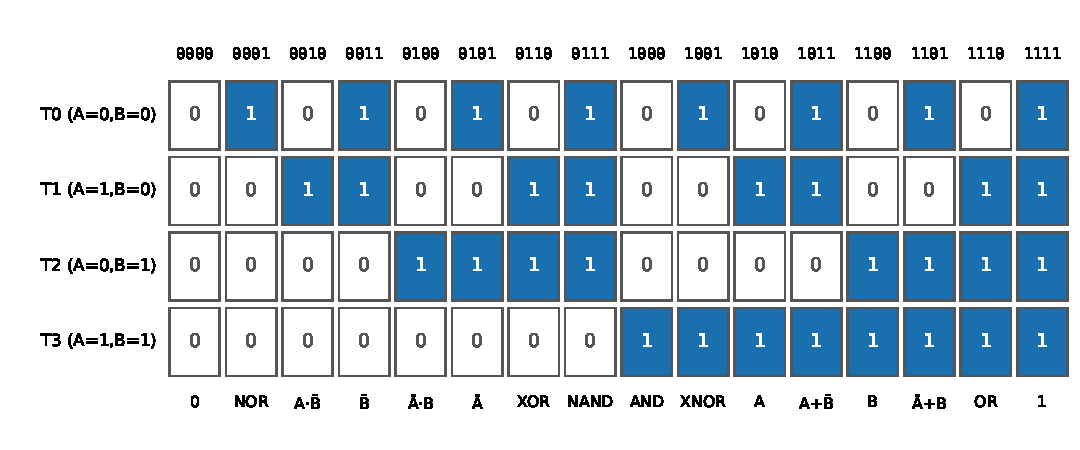
\includegraphics[width=\textwidth]{fig_truth_tables.pdf}
\caption{All 16 Boolean functions of two inputs, each as its truth
table of four bits $T_0\ldots T_3$. The row index is $2B+A$, so $T_0$ is
the output for $A=B=0$ and $T_3$ for $A=B=1$. Written as the 4-bit
number $T_3T_2T_1T_0$, the functions are simply the numbers 0 to 15.
A LUT stores one such column.}
\label{fig:truth_tables}
\end{figure}

We fix a convention for the rest of the text. The four bits of the table
are named $T_0$ to $T_3$, and the row that the inputs select has the
index
\begin{equation}
    i = 2B + A,
    \label{eq:index}
\end{equation}
so that $A$ is the least significant bit of the index and $B$ the most
significant. Written as a binary number $T_3T_2T_1T_0$, every function
is a number between 0 and 15: XOR is $0110_2=6$, AND is $1000_2=8$, NAND
is $0111_2=7$.

\subsection{The idea: store, do not compute}

Here is the whole idea of the look-up table in one sentence: if a
function is its truth table, then a circuit that stores the truth table
and lets the inputs select a row \emph{is} the function. Formally,
\begin{equation}
    Y = T_{2B+A}.
    \label{eq:lut}
\end{equation}
The circuit does not know what AND or XOR is. It knows four bits and an
index. Change the four bits, and the same hardware is a different gate.

\begin{merke}
A look-up table with $k$ inputs is $2^k$ stored bits and a selector.
It realises every one of the $2^{2^k}$ functions of $k$ inputs, and
which one is decided by the stored bits alone. The stored bits are its
\emph{configuration}.
\end{merke}

This is a trade. A dedicated AND gate in CMOS needs six transistors; a
LUT that can be an AND gate, as we will see, needs twenty plus the
memory. In exchange one gets a circuit whose function can be set after
manufacture, and this is what an FPGA is made of. The first commercial
FPGA, the Xilinx XC2064 of 1985, used look-up tables with four inputs
as its logic element~\cite{Carter1986,Freeman1989}; the choice of a
LUT, rather than a fixed set of gates, was later shown to be close to
optimal in area for LUTs of four to six inputs~\cite{Rose1990,Ahmed2004}.

% ============================================================
\section{The selector: a tree of multiplexers}
\label{sec:mux}
% ============================================================

\subsection{The 2:1 multiplexer}

The simplest selector is the 2:1 multiplexer: two data inputs $I_0$ and
$I_1$, one select input $S$, one output. Its function is
\begin{equation}
    \mathrm{MUX}(I_0,I_1,S) = \begin{cases} I_0 & \text{if } S=0,\\
                                             I_1 & \text{if } S=1,\end{cases}
    \qquad\text{or}\qquad
    \mathrm{MUX} = \ovl{S}\cdot I_0 + S\cdot I_1 .
    \label{eq:mux}
\end{equation}
In words: exactly one of two paths is connected to the output, and $S$
decides which. This is a description that invites a mechanical picture.
A multiplexer is two switches that share their output; the first is
closed when $S=0$, the second when $S=1$; never both, never neither.
We will build it exactly this way in Section~\ref{sec:switch}.

\subsection{Shannon's expansion: the tree is forced}

How does one select one of four bits with two select signals? One could
imagine many arrangements. There is a theorem that says the natural
one is the only one needed. Shannon's expansion
theorem~\cite{Shannon1938,Shannon1949} states that every Boolean
function can be split with respect to one of its variables:
\begin{equation}
    f(A,B) = \ovl{B}\cdot f(A,0) + B\cdot f(A,1).
    \label{eq:shannon}
\end{equation}
The proof is two lines: if $B=0$ the right side is $1\cdot f(A,0)+0$,
which is $f(A,0)$; if $B=1$ it is $0+1\cdot f(A,1)$, which is $f(A,1)$.
In both cases it equals $f(A,B)$.

Now compare equation~\eqref{eq:shannon} with
equation~\eqref{eq:mux}. They have the same shape: the right side of
Shannon's expansion \emph{is} a 2:1 multiplexer with select input $B$,
data input $I_0 = f(A,0)$ and data input $I_1 = f(A,1)$. The two data
inputs are themselves functions, of one variable fewer. We expand them
in turn.

\begin{rechnung}
\textbf{Step 1 -- expand with respect to $B$.} By
equation~\eqref{eq:shannon},
\begin{equation*}
    f(A,B) = \mathrm{MUX}\bigl(f(A,0),\, f(A,1),\, B\bigr).
\end{equation*}
This is one multiplexer whose select input is $B$. Its outputs we call
$N_0 = f(A,0)$ and $N_1 = f(A,1)$ in the circuit.

\textbf{Step 2 -- expand $N_0$ with respect to $A$.} The function
$f(A,0)$ has one input left. Applying the theorem to it,
\begin{equation*}
    f(A,0) = \ovl{A}\cdot f(0,0) + A\cdot f(1,0)
           = \mathrm{MUX}\bigl(f(0,0),\, f(1,0),\, A\bigr).
\end{equation*}
The data inputs $f(0,0)$ and $f(1,0)$ are no longer functions: they are
constants, the two table entries $T_0$ and $T_1$.

\textbf{Step 3 -- expand $N_1$ with respect to $A$.} In the same way
\begin{equation*}
    f(A,1) = \mathrm{MUX}\bigl(f(0,1),\, f(1,1),\, A\bigr)
           = \mathrm{MUX}(T_2, T_3, A).
\end{equation*}

\textbf{Step 4 -- read off the index.} The output is $T_i$ with
$i=f(0,0)\to0$, $f(1,0)\to1$, $f(0,1)\to2$, $f(1,1)\to3$, that is
$i=2B+A$: $B$ chose between the upper and the lower pair, $A$ chose
within the pair. This is equation~\eqref{eq:index}.
\end{rechnung}

The result is Figure~\ref{fig:mux_tree}: three 2:1 multiplexers in a
tree, two at the first level selected by $A$, one at the second level
selected by $B$. The leaves of the tree are the four stored bits. Every
LUT in every FPGA has this structure, with as many levels as inputs,
because Shannon's expansion leaves no freedom: once one decides to
store the truth table, the selector is a multiplexer tree. What remains
to be decided is only what the switches are made of.

\begin{figure}[H]
\centering
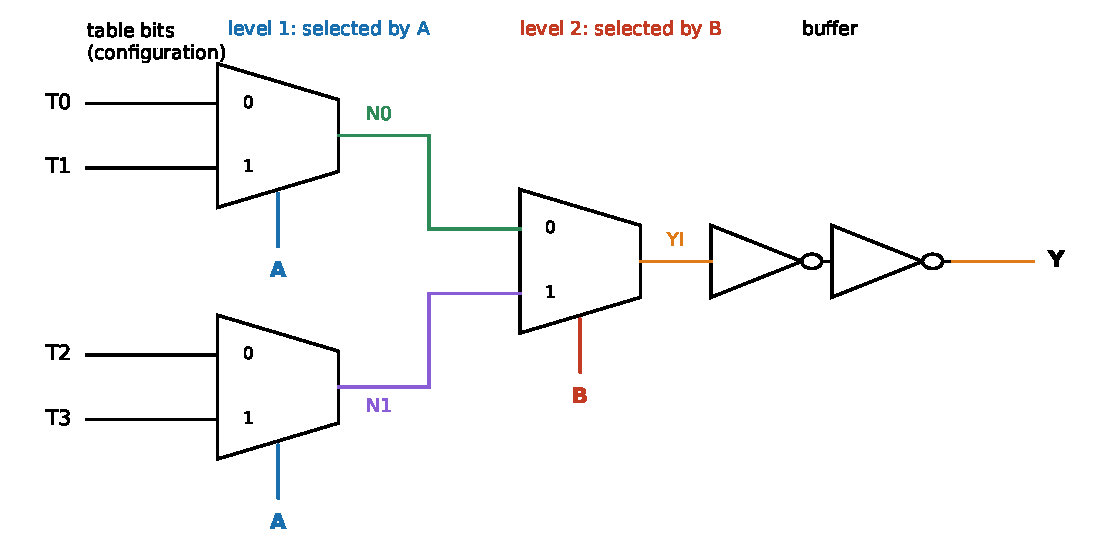
\includegraphics[width=0.9\textwidth]{fig_mux_tree.pdf}
\caption{The LUT with two inputs as a tree of 2:1 multiplexers. The
first level, selected by $A$, chooses within the pairs $(T_0,T_1)$ and
$(T_2,T_3)$; the second level, selected by $B$, chooses between the
pairs. The two inverters at the output are the buffer of
Section~\ref{sec:inverter}.}
\label{fig:mux_tree}
\end{figure}

\begin{merke}
Shannon's expansion $f(A,B)=\ovl B\,f(A,0)+B\,f(A,1)$ is a 2:1
multiplexer. Applied once per input, it turns every function of $k$
inputs into a tree of $2^k-1$ multiplexers whose leaves are the $2^k$
bits of the truth table. The LUT is this theorem, built.
\end{merke}

A small point that will matter in Section~\ref{sec:glitch}: the
multiplexer tree is a \emph{path}. At any moment exactly one of the
four stored bits is connected, through two closed switches, to the
output. When an input changes, one switch opens and another closes, and
for a short time the output is connected to nothing, or to a node that
still carries the old value. The tree is a selector of wires, not a
computation of values, and this has consequences in time.

% ============================================================
\section{The switch: a MOS transistor}
\label{sec:switch}
% ============================================================

\subsection{The MOSFET as a switch}

The metal-oxide-semiconductor field-effect transistor was patented by
Lilienfeld in 1930 as an idea~\cite{Lilienfeld1930} and first made to
work by Kahng and Atalla in 1960~\cite{Kahng1960}. It has three
terminals that matter here, gate, drain and source, and a fourth, the
bulk, that we will need in a moment. For our purposes it is a switch
between drain and source that is controlled by the voltage on the gate.
An n-channel transistor (NMOS) conducts when its gate is at a higher
voltage than its source by more than the \textbf{threshold voltage}
$\VT$; a p-channel transistor (PMOS) conducts when its gate is
\emph{lower} than its source by more than $|\VT|$.

To calculate anything we need a model. We use the simplest one, the
level-1 model of Shichman and Hodges~\cite{Shichman1968}, which is the
model that SPICE~\cite{Nagel1973} and therefore ngspice evaluate when
the netlist says \texttt{level=1}. For an NMOS with gate-source voltage
$V_{GS}$ and drain-source voltage $V_{DS}$ the drain current is
\begin{equation}
    I_D = \begin{cases}
        0 & V_{GS}\le\VT \quad\text{(off)},\\[2pt]
        k\Bigl[(V_{GS}-\VT)\,V_{DS} - \tfrac12 V_{DS}^2\Bigr]
            & V_{DS} < V_{GS}-\VT \quad\text{(linear)},\\[2pt]
        \tfrac{k}{2}\,(V_{GS}-\VT)^2
            & V_{DS}\ge V_{GS}-\VT \quad\text{(saturation)},
    \end{cases}
    \label{eq:level1}
\end{equation}
with the transconductance parameter $k = k'\,W/L$. The transistors of
this text have $W=L=\SI{10}{\micro m}$, so $k=k'$, and the numbers are
\begin{center}
\begin{tabular}{lcccc}
\toprule
 & $\VT$ & $k'$ & $\gamma$ & $\phi$ \\
\midrule
NMOS & \SI{1.0}{V} & \SI{1.0}{mA/V^2} & \SI{0.4}{V^{1/2}} & \SI{0.65}{V} \\
PMOS & \SI{-1.0}{V} & \SI{0.5}{mA/V^2} & \SI{0.4}{V^{1/2}} & \SI{0.65}{V} \\
\bottomrule
\end{tabular}
\end{center}
The PMOS has half the transconductance because holes are less mobile
than electrons; the ratio of two to three is typical of silicon. The
supply voltage is $\VDD=\SI{5}{V}$. These numbers describe no
particular part or process; they are chosen to be plausible, and all
delays in Section~\ref{sec:simulation} are properties of these numbers.

In the linear region, for small $V_{DS}$, equation~\eqref{eq:level1}
says that the transistor is a resistor:
\begin{equation}
    R_{on} = \frac{V_{DS}}{I_D} \approx \frac{1}{k\,(V_{GS}-\VT)}
           = \frac{1}{\SI{1}{mA/V^2}\cdot(\SI{5}{V}-\SI{1}{V})}
           = \SI{250}{\ohm}
    \label{eq:ron}
\end{equation}
for an NMOS with its gate at $\VDD$ and its source at ground. This is
what a closed switch looks like from the outside: a few hundred ohms.
The PMOS with its gate at ground and its source at $\VDD$ has twice that,
\SI{500}{\ohm}.

\subsection{Why one NMOS is not enough: the lost threshold}
\label{sec:pass}

Take a single NMOS as the switch of the multiplexer. Its gate is the
select signal, at \SI{5}{V} when the switch should be closed; its two
other terminals are the input and the output of the switch, and which
of them is drain and which is source is decided by the voltages:
the source is the terminal at the lower potential.

\emph{Passing a 0.} The input is at \SI{0}{V} and the output node, say,
charged to \SI{5}{V}. The input is the source, $V_{GS}=\SI{5}{V}$, the
transistor is on with $R_{on}=\SI{250}{\ohm}$, and the output
discharges all the way to \SI{0}{V}. Nothing stops it: $V_{GS}$ stays
at \SI{5}{V} throughout.

\emph{Passing a 1.} The input is at \SI{5}{V} and the output at
\SI{0}{V}. Now the output is the source, because it is lower. At first
$V_{GS}=\SI{5}{V}$ and the output charges quickly. But as the output
rises, $V_{GS}$ falls: the gate stays at \SI{5}{V}, the source
climbs. When the output reaches $\VDD-\VT$, $V_{GS}=\VT$ and the
transistor turns off. The output never reaches \SI{5}{V}; it stops one
threshold short.

It is worse than that, because $\VT$ is not a constant. In the level-1
model the threshold depends on the voltage between source and bulk,
$V_{SB}$, through the \textbf{body effect}:
\begin{equation}
    \VT(V_{SB}) = V_{T0} + \gamma\Bigl(\sqrt{\phi+V_{SB}} - \sqrt{\phi}\Bigr).
    \label{eq:body}
\end{equation}
The bulk of every NMOS is tied to ground, as on a chip. When the source
rises to several volts, $V_{SB}$ is several volts, and the threshold
rises with it.

\begin{rechnung}
\textbf{Step 1 -- the condition.} The output voltage $V$ stops rising
when $V_{GS}$ has fallen to the threshold, that is when
$\VDD - V = \VT(V)$, with $V_{SB}=V$ because the bulk is at ground:
\begin{equation*}
    V = \VDD - V_{T0} - \gamma\Bigl(\sqrt{\phi+V}-\sqrt{\phi}\Bigr).
\end{equation*}

\textbf{Step 2 -- first guess without body effect.} With $\gamma=0$ the
answer would be $V=\SI{5}{V}-\SI{1}{V}=\SI{4}{V}$.

\textbf{Step 3 -- iterate.} Insert $V=\SI{4}{V}$ on the right:
$\sqrt{0.65+4}=2.156$, $\sqrt{0.65}=0.806$, difference $1.350$, times
$\gamma$ gives \SI{0.540}{V}. So $V = 4 - 0.540 = \SI{3.46}{V}$. Insert
again: $\sqrt{4.11}=2.027$, difference $1.221$, times $\gamma$ is
\SI{0.488}{V}, so $V=\SI{3.51}{V}$. One more round changes the third
decimal only.

\textbf{Step 4 -- result.} A single NMOS with its gate at \SI{5}{V}
passes a 1 as
\begin{equation*}
    V_{max} \approx \SI{3.51}{V},
\end{equation*}
\SI{1.49}{V} below the supply. The threshold at that point is
$\VT(\SI{3.51}{V})=\SI{1.49}{V}$, half again as large as $V_{T0}$.
\end{rechnung}

Figure~\ref{fig:pass_level} shows both halves of this calculation. The
number \SI{3.51}{V} is well above half the supply, so a following
inverter would still read it as a~1. But an inverter whose input sits
at \SI{3.5}{V} is not fully switched; we will see in
Section~\ref{sec:inverter} that it then draws a continuous current.
And a second NMOS switch in series, as in the second level of the
tree, would start from \SI{3.51}{V} and lose nothing further, since the
threshold condition is the same, but it would charge its output more
slowly, because it operates with less gate drive. Pass-transistor
LUTs exist and are common in FPGAs, where area is precious and the
level is restored by a dedicated circuit; for a circuit that should be
understood rather than minimised, the cleaner choice is the next one.

\begin{figure}[H]
\centering
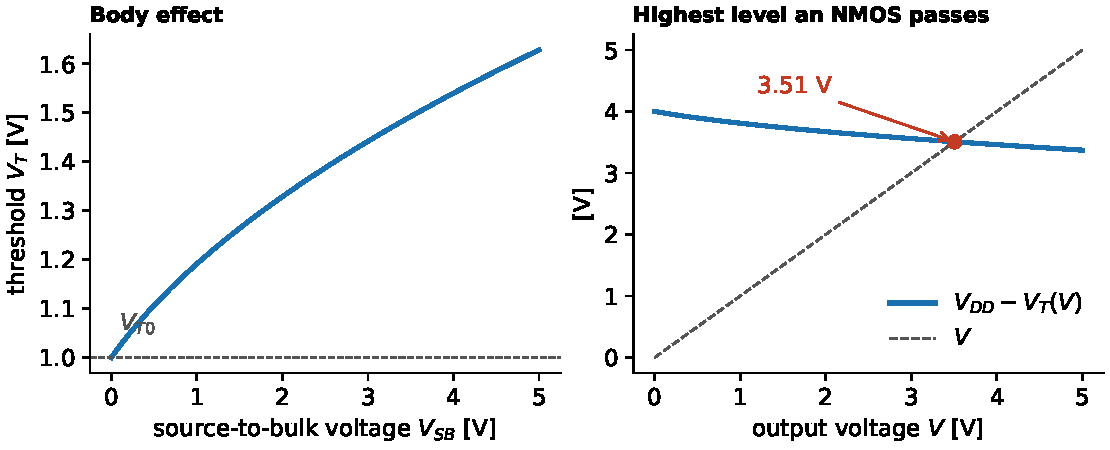
\includegraphics[width=\textwidth]{fig_pass_level.pdf}
\caption{Left: the threshold of the NMOS rises with the source-to-bulk
voltage (body effect, equation~\eqref{eq:body}). Right: the output of
an NMOS switch passing a~1 stops where $V=\VDD-\VT(V)$, at
\SI{3.51}{V} for these transistors. Computed from the model
parameters in \texttt{lut.py}.}
\label{fig:pass_level}
\end{figure}

\subsection{The transmission gate}

The PMOS has the mirror-image problem. With its gate at \SI{0}{V} it
passes a~1 perfectly, because its source is then the \SI{5}{V} side and
$V_{SG}$ stays at \SI{5}{V} throughout; but it cannot pull a node below
$|\VT|$ above ground, for the same reason the NMOS cannot pull a node
above $\VDD-\VT$.

The solution is to use both. An NMOS and a PMOS in parallel, the NMOS
gate driven by the select signal $S$ and the PMOS gate by its complement
$\ovl S$, form the \textbf{transmission gate}
(Figure~\ref{fig:sch_switch}). When $S=1$ both transistors are on. For
a~0 the NMOS does the work and the PMOS helps until the node is
within $|\VT|$ of ground; for a~1 the PMOS does the work and the NMOS
helps until the node is within $\VT$ of the supply. The node reaches
both rails exactly. When $S=0$ both transistors are off and the switch
is open.

\begin{figure}[H]
\centering
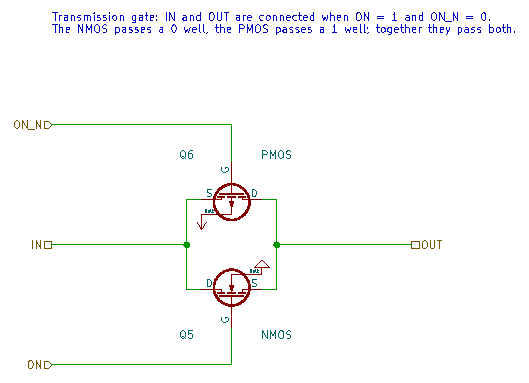
\includegraphics[width=0.55\textwidth]{sch_lut2-mux_n0-sw0.pdf}
\caption{The switch sheet of the schematic: one transmission gate. The
NMOS (bottom) is driven by \texttt{ON}, the PMOS (top) by
\texttt{ON\_N}. \texttt{IN} and \texttt{OUT} are interchangeable; the
switch conducts in both directions. The bulk of the NMOS is at ground,
that of the PMOS at the supply.}
\label{fig:sch_switch}
\end{figure}

The on-resistance of the transmission gate is the parallel combination
of the two. At the midpoint of the swing, $V=\SI{2.5}{V}$, both
transistors see a gate drive of about \SI{2.5}{V} minus a threshold of
about \SI{1.3}{V} with body effect; the NMOS contributes roughly
$1/(\SI{1}{mA/V^2}\cdot\SI{1.2}{V})\approx\SI{0.8}{k\ohm}$ and the PMOS
about twice that, in parallel some \SI{550}{\ohm}. Near the rails one
transistor takes over, with $R_{on}$ of a few hundred ohms. The
transmission gate is, to a fair approximation, a resistor of a few
hundred ohms that is independent of the level it passes.

The price is two transistors per switch instead of one, and a
complement of each select signal. In the LUT the select signals are the
inputs $A$ and $B$, so two inverters produce $\ovl A$ and $\ovl B$; they
appear on the root sheet of the schematic. Each 2:1 multiplexer is two
transmission gates, one driven by $(S,\ovl S)$ and one by
$(\ovl S, S)$, so that exactly one is closed
(Figure~\ref{fig:sch_mux}).

\begin{figure}[H]
\centering
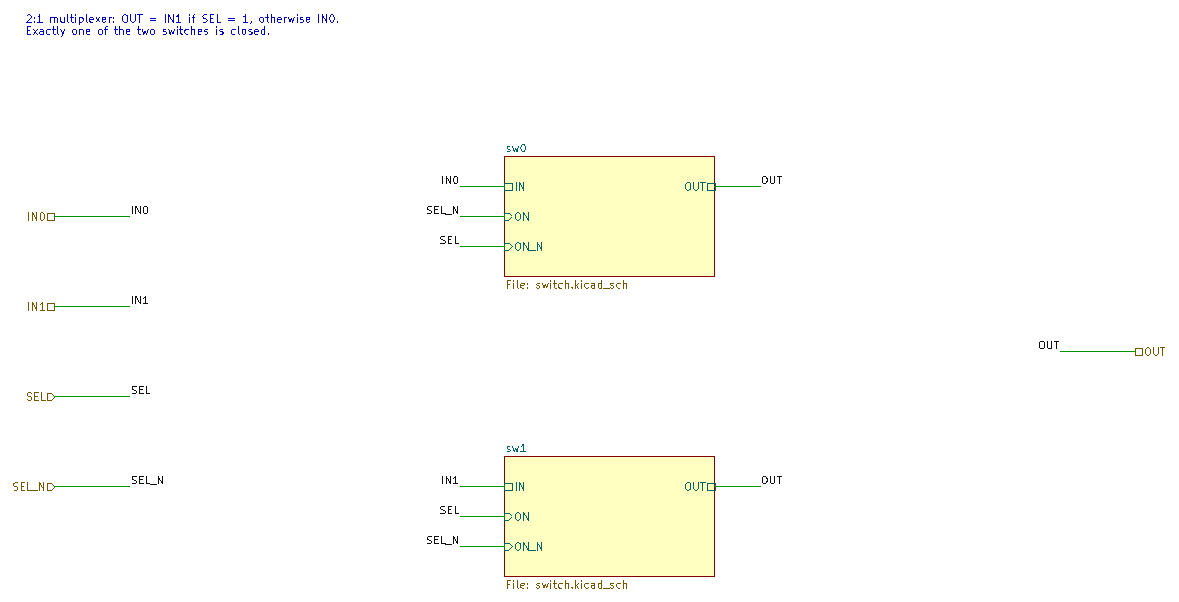
\includegraphics[width=0.8\textwidth]{sch_lut2-mux_n0.pdf}
\caption{The multiplexer sheet: two switches that share their output.
\texttt{sw0} is closed when \texttt{SEL} $=0$, \texttt{sw1} when
\texttt{SEL} $=1$. The sheet is used three times in the LUT.}
\label{fig:sch_mux}
\end{figure}

\begin{merke}
An NMOS passes a~0 well and a~1 only up to $\VDD-\VT$, which with the
body effect is \SI{3.51}{V} here; a PMOS has the opposite limitation.
In parallel, driven by complementary signals, they pass both levels in
full: this is the transmission gate, the switch of this LUT. It costs
two transistors and the complement of the select signal.
\end{merke}

% ============================================================
\section{The inverter and the output buffer}
\label{sec:inverter}
% ============================================================

\subsection{The CMOS inverter}

The complementary MOS inverter, proposed by Wanlass and Sah in
1963~\cite{Wanlass1963}, is one PMOS above one NMOS
(Figure~\ref{fig:sch_inverter}). Both gates are the input, both drains
are the output, the PMOS source is at $\VDD$ and the NMOS source at
ground. For an input of~0 the NMOS is off and the PMOS is on: the
output is pulled to $\VDD$ through the PMOS, and no current flows,
because the path to ground is open. For an input of~1 the roles swap.
In either steady state one of the two transistors is off, and the
circuit draws no current. This was the point of Wanlass's paper, whose
title promised nanowatt logic, and it is the reason CMOS won.

\begin{figure}[H]
\centering
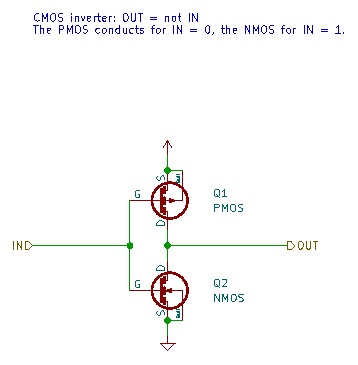
\includegraphics[width=0.5\textwidth]{sch_lut2-inv_a.pdf}
\caption{The inverter sheet: one PMOS, one NMOS, sources and bulks at
the rails. It is used four times: twice for $\ovl A$ and $\ovl B$ on
the root sheet and twice in the output buffer.}
\label{fig:sch_inverter}
\end{figure}

\subsection{The switching threshold}

Between the two steady states, for an input somewhere in the middle,
both transistors conduct. The input voltage at which the output equals
the input is the \textbf{switching threshold} $V_M$; it is the voltage
that the inverter regards as the boundary between~0 and~1. We can
compute it from equation~\eqref{eq:level1}.

\begin{rechnung}
\textbf{Step 1 -- both transistors in saturation.} At $V_{in}=V_{out}=V_M$
the NMOS has $V_{GS}=V_{DS}=V_M$, so $V_{DS}\ge V_{GS}-\VT$ and it is
saturated. The PMOS has $V_{SG}=V_{SD}=\VDD-V_M$ and is saturated too.

\textbf{Step 2 -- equal currents.} No current leaves at the output, so
the drain currents are equal:
\begin{equation*}
    \frac{k_n}{2}\,(V_M - V_{Tn})^2 = \frac{k_p}{2}\,(\VDD - V_M - |V_{Tp}|)^2 .
\end{equation*}

\textbf{Step 3 -- take the square root.} Both sides are positive, so
\begin{equation*}
    \sqrt{k_n}\,(V_M - V_{Tn}) = \sqrt{k_p}\,(\VDD - V_M - |V_{Tp}|).
\end{equation*}

\textbf{Step 4 -- solve for $V_M$.} Collecting terms with
$r=\sqrt{k_p/k_n}$,
\begin{equation}
    V_M = \frac{V_{Tn} + r\,(\VDD - |V_{Tp}|)}{1 + r}.
    \label{eq:vm}
\end{equation}

\textbf{Step 5 -- numbers.} $r=\sqrt{0.5}=0.707$, so
\begin{equation*}
    V_M = \frac{1 + 0.707\cdot(5-1)}{1.707}\,\si{V} = \frac{3.83}{1.707}\,\si{V}
        = \SI{2.24}{V}.
\end{equation*}
\end{rechnung}

The threshold is below half the supply because the PMOS is the weaker
transistor: it takes a lower input, and therefore a stronger PMOS
drive, to balance the NMOS. A symmetric inverter would have the PMOS
twice as wide; we have not done that, and $V_M=\SI{2.24}{V}$ is the
consequence. Figure~\ref{fig:inverter_vtc} shows the full transfer
curve, obtained by solving the current balance numerically for every
input voltage, and next to it the current through the inverter. The
current is zero at both rails and peaks at $V_M$, where both
transistors are saturated with a gate drive of about \SI{1.2}{V}:
$I=\tfrac12\cdot\SI{1}{mA/V^2}\cdot(1.24)^2\approx\SI{0.77}{mA}$.

\begin{figure}[H]
\centering
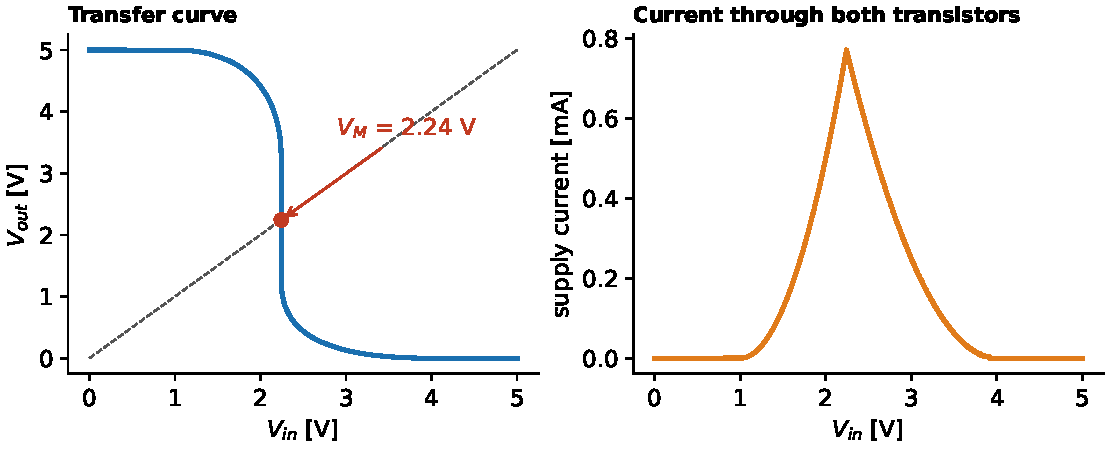
\includegraphics[width=\textwidth]{fig_inverter_vtc.pdf}
\caption{Left: the static transfer curve of the inverter from the
level-1 model, with the switching threshold $V_M=\SI{2.24}{V}$ where
the curve crosses the diagonal. Right: the current through the two
transistors. It is zero when the input is at a rail and
\SI{0.77}{mA} at $V_M$. An input that rests between the rails costs
current.}
\label{fig:inverter_vtc}
\end{figure}

This figure explains why the lost threshold of Section~\ref{sec:pass}
would have mattered. An inverter whose input rests at \SI{3.5}{V}
instead of \SI{5}{V} sits on the right flank of the current curve, at
roughly \SI{0.1}{mA}; a LUT built from single pass transistors
therefore draws a static current whenever its output is~1, and the
circuit of this text, whose inverter inputs reach the rails, draws
none.

\subsection{Why two inverters}

The output of the multiplexer tree, the node $YI$, is a stored bit seen
through two transmission gates. It carries the right level, but it is
a weak node: its source is a stored bit, in an FPGA a tiny memory cell,
and it is connected through some \SI{500}{\ohm} of switch. Asking it to
drive a load would be asking the memory to drive the load. So the
tree's output is \textbf{buffered}: the first inverter reads $YI$ and
produces its complement with the full strength of its own transistors;
the second inverter restores the polarity and drives the load
(Figure~\ref{fig:sch_buffer}). The first inverter also \emph{restores}
the level, in the sense that whatever is between the rails at its
input becomes a clean rail at its output; this is why it is called a
restoring stage, and why it would also have rescued a pass-transistor
tree, at the cost of the static current just computed.

\begin{figure}[H]
\centering
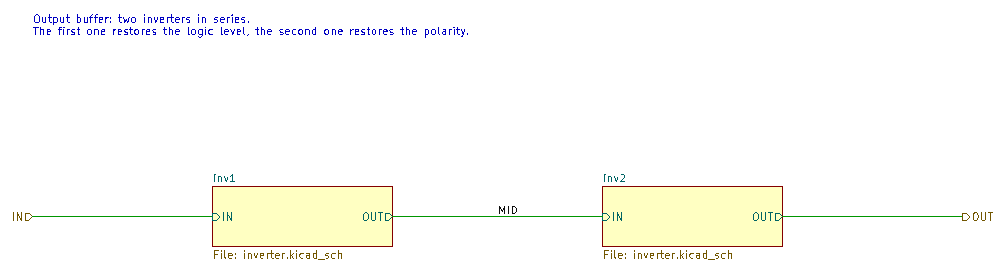
\includegraphics[width=0.75\textwidth]{sch_lut2-buffer.pdf}
\caption{The buffer sheet: two inverters in series. \texttt{MID} is
the inverted, restored signal; \texttt{OUT} drives the load.}
\label{fig:sch_buffer}
\end{figure}

\begin{merke}
A CMOS inverter draws no current at rest and switches at
$V_M=(V_{Tn}+r(\VDD-|V_{Tp}|))/(1+r)$, here \SI{2.24}{V}. Two of them
in series restore the level of the multiplexer tree, restore its
polarity, and drive the load with their own transistors instead of
with the stored bit.
\end{merke}

% ============================================================
\section{The complete circuit}
\label{sec:circuit}
% ============================================================

\subsection{Twenty transistors}

We can now count. The tree has three multiplexers of two transmission
gates each, six switches of two transistors: twelve. The complements
$\ovl A$ and $\ovl B$ are two inverters: four. The buffer is two
inverters: four. In total,
\begin{equation}
    12 + 4 + 4 = 20 \text{ transistors},
\end{equation}
ten NMOS and ten PMOS. Figure~\ref{fig:sch_root} shows the root sheet
of the schematic, with the four stored bits, the inverters for the
complements, the three multiplexers and the buffer.

\begin{figure}[H]
\centering
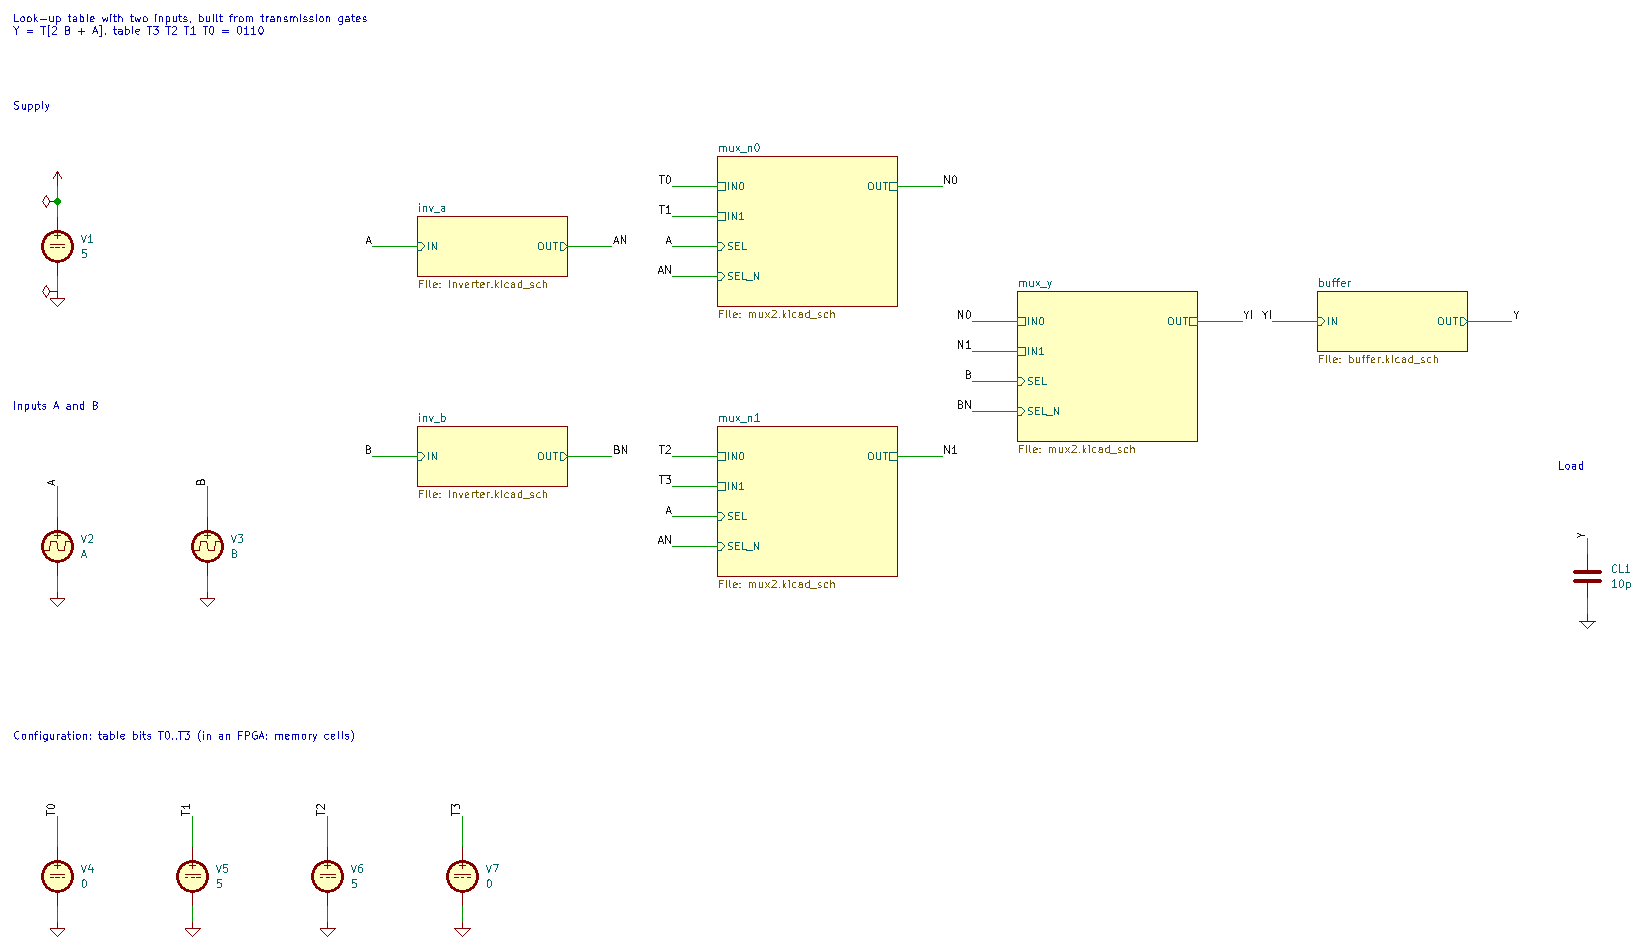
\includegraphics[width=\textwidth]{sch_lut2.pdf}
\caption{The root sheet of the LUT. Left: the supply, the two inputs
$A$ and $B$ as pulse sources, and the four configuration sources
$T_0\ldots T_3$. Middle: the inverters \texttt{inv\_a} and
\texttt{inv\_b} for the complements, the two first-level multiplexers
\texttt{mux\_n0} and \texttt{mux\_n1} selected by $A$, and
\texttt{mux\_y} selected by $B$. Right: the buffer and the load of
\SI{10}{pF}. In this instance the table is $0110$, XOR.}
\label{fig:sch_root}
\end{figure}

The schematic is hierarchical: every building block is drawn once, on
a sheet of its own, and used as often as needed. Five sheet files
describe fifteen sheet instances:

\begin{center}
\begin{tabular}{llll}
\toprule
Sheet & Content & Used & Transistors \\
\midrule
\texttt{lut2} & sources, load, and the sheets below & 1 & -- \\
\texttt{inverter} & one PMOS, one NMOS & 4 & 2 each \\
\texttt{mux2} & two switches & 3 & -- \\
\texttt{switch} & one transmission gate & 6 & 2 each \\
\texttt{buffer} & two inverters & 1 & -- \\
\bottomrule
\end{tabular}
\end{center}

The hierarchy is three levels deep: the transistors of a switch sit in
\texttt{lut2 / mux\_n0 / sw0}. The schematic is not drawn by hand. It is
written by a Python program, from the same description that generates
the SKiDL netlist, and the two are checked against each other: the
netlist that KiCad extracts from the drawn sheets must have exactly
the same connectivity as the netlist that SKiDL built in memory. That
check passes, and it is the reason we can trust that the figures in
this text show the circuit that was simulated.

\subsection{Configuration by voltage sources}

The four stored bits are the configuration of the LUT. In an FPGA they
are memory cells, static RAM in nearly all devices since the
XC2064~\cite{Carter1986}, written once when the bitstream is loaded and
then holding their value for as long as the power is on. The LUT does
not care where the bits come from; it only needs four nodes that are
at a~0 or a~1.

In this text the four bits are \textbf{voltage sources}: \SI{0}{V} for
a~0, \SI{5}{V} for a~1. This choice has two advantages for
understanding. First, the configuration is visible in the schematic:
the four source values on the root sheet \emph{are} the function, and
one can read XOR off Figure~\ref{fig:sch_root} by reading the sources
$T_3T_2T_1T_0=0110$. Second, the simulation can change the function at
will, simply by changing the source waveforms, and so one run can
cover all 16 functions. What one gives up is realism in one respect:
a voltage source has no output resistance and is never disturbed by
the circuit it drives. A memory cell is, and in an FPGA the cells and
the switches are dimensioned together so that reading the cell through
the tree never flips it. That is a question of sizing, not of
function, and we leave it aside.

\begin{merke}
The LUT with two inputs is 20 transistors: twelve in six transmission
gates, four in the inverters that complement the inputs, four in the
output buffer. Its configuration is four bits, here four voltage
sources, in an FPGA four memory cells. The circuit is the same for all
16 functions; only the four bits differ.
\end{merke}

% ============================================================
\section{Simulation}
\label{sec:simulation}
% ============================================================

\subsection{The toolchain}

The circuit is described in Python with SKiDL~\cite{SKiDL}, a library
that builds a netlist from Python objects. A small hierarchy layer
turns the description into KiCad sheets and places the symbols;
KiCad's command-line tool extracts a flat SPICE netlist from the drawn
schematic, so that what is simulated is the drawing, not the Python.
The netlist is simulated with ngspice~\cite{ngspice}, the open-source
descendant of SPICE~\cite{Nagel1973}, in a transient analysis with a
step of \SI{0.2}{ns}. The node voltages are written to a value change
dump (VCD) file~\cite{IEEE1364}, the waveform format of digital
simulators, which also accepts real-valued signals, and viewed in
GTKWave. Delays, levels and currents are extracted with NumPy. All of
this runs from two commands and takes a few seconds.

\subsection{The stimulus}

One run should cover all 16 functions. The inputs $A$ and $B$ step
through their four combinations in \SI{200}{ns} steps, and every
\SI{800}{ns} the four table sources are rewritten to the next
function, $f=0,1,\ldots,15$. The order of the input combinations is
not $00,01,10,11$ but the Gray code $00,10,11,01$, index $0,1,3,2$, in
which exactly one input changes per step~\cite{Gray1953}. This is
deliberate: when only one input changes, every edge of the output can
be attributed to that input, and the delay from that input to the
output can be measured. The table is rewritten \SI{100}{ns} into each
window, while both inputs are~0, so that the rewrite is visible as a
change of the output that has nothing to do with the inputs.

The output is sampled \SI{5}{ns} before the end of every step and
compared with the table bit that the index selects. Sixty-four samples,
four per function, make up the measured truth tables.

\subsection{Result: all 16 functions}

Figure~\ref{fig:xor} shows one function window, the one in which the
table is XOR. At \SI{100}{ns} the sources change from $0101$ ($\ovl A$)
to $0110$; the output, which was~1 at index~0 for $\ovl A$, falls to~0,
because $T_0$ of XOR is~0. Then the index steps through $1,3,2$ and the
output shows $1,0,1$: $T_1=1$, $T_3=0$, $T_2=1$, the truth table of
XOR. The middle panel shows how the tree does it: $N_0$ is $T_0$ or
$T_1$ depending on $A$, $N_1$ is $T_2$ or $T_3$, and $YI$ follows
whichever of them $B$ selects.

\begin{figure}[H]
\centering
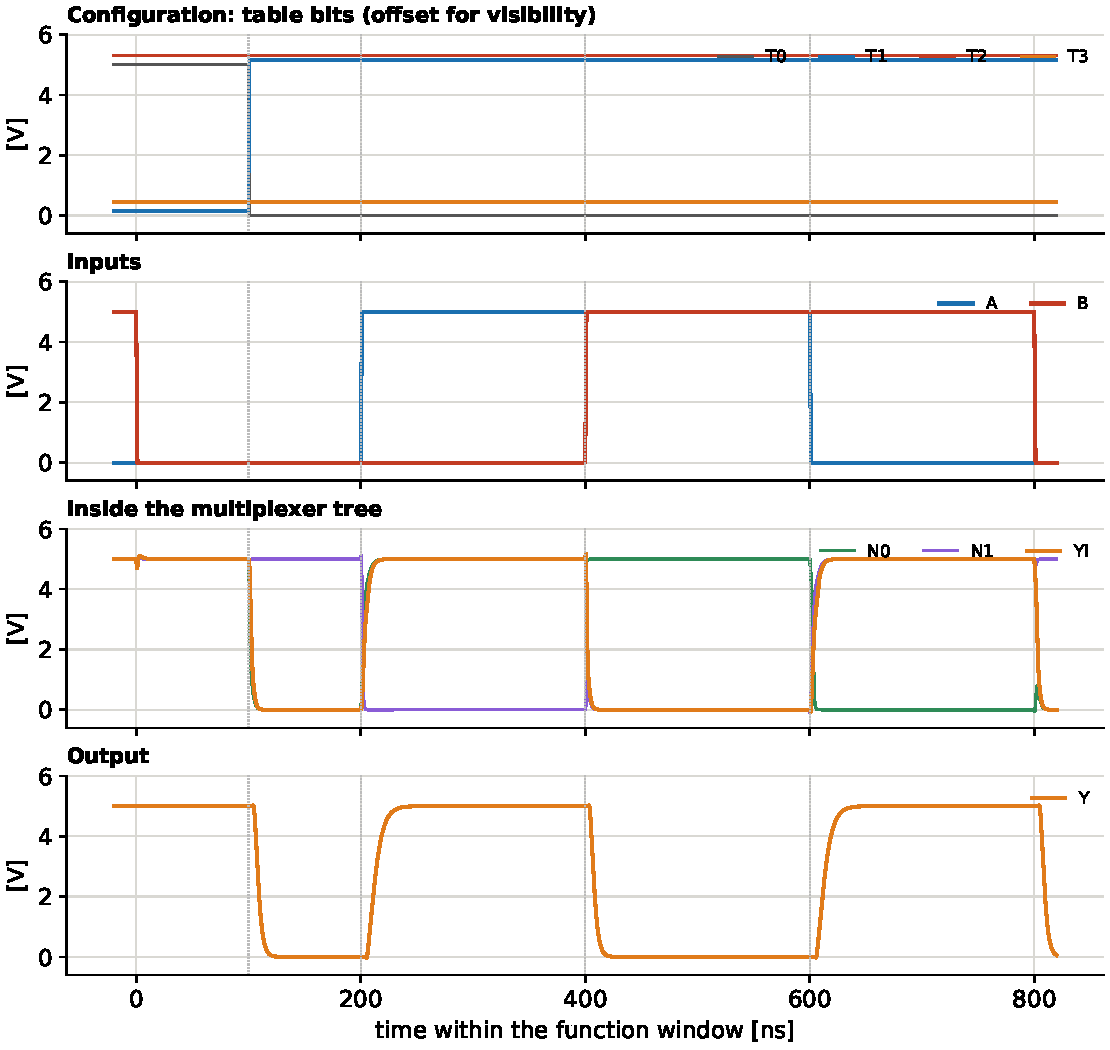
\includegraphics[width=\textwidth]{fig_xor.pdf}
\caption{One function window of the simulation, \SI{800}{ns} long,
with the table configured as XOR at \SI{100}{ns}. Top: the four
configuration sources (vertically offset so that they can be told
apart). Second: the inputs in Gray code. Third: the nodes of the tree;
$N_0$ and $N_1$ are the outputs of the first level, $YI$ the output of
the second. Bottom: the output $Y$ after the buffer. Dotted lines mark
the rewrite and the input changes.}
\label{fig:xor}
\end{figure}

The other fifteen windows look the same with other patterns. The
measured truth tables agree with the configured ones in all 64
entries. The internal node $YI$ reaches \SI{5.000}{V} for every~1 and
\SI{0.0}{mV} for every~0, as the transmission gates promised; the
output reaches \SI{5.000}{V}; and the supply current at rest, measured
in the last \SI{20}{ns} of every step, is at most \SI{0.015}{\micro A},
which is the leakage of the junction capacitances in the model and
confirms that no inverter is stuck between the rails.

\subsection{Delays}
\label{sec:delays}

The delay from an input edge to the following output edge, measured
from half-supply crossing to half-supply crossing, is listed in
Table~\ref{tab:delays}. Each number is the mean over the eight edges
of that kind in the run.

\begin{table}[H]
\centering
\caption{Propagation delays, 50\,\% to 50\,\%, with a load of
\SI{10}{pF}. From \texttt{results/summary.md}.}
\label{tab:delays}
\begin{tabular}{lcc}
\toprule
From & to $Y$ rising & to $Y$ falling \\
\midrule
input $A$ & \SI{12.2}{ns} & \SI{9.1}{ns} \\
input $B$ & \SI{10.8}{ns} & \SI{7.8}{ns} \\
a table bit & \SI{11.1}{ns} & \SI{8.2}{ns} \\
\bottomrule
\end{tabular}
\end{table}

Three things can be read from this table, and all three can be
understood from the model.

\emph{Rising is slower than falling.} The last inverter charges the
\SI{10}{pF} load through its PMOS and discharges it through its NMOS,
and the PMOS has half the transconductance. The difference of about
\SI{3}{ns} is this asymmetry.

\emph{$B$ is faster than $A$.} A change of $A$ switches the first
level of the tree; the new value must then pass through the second
level as well. A change of $B$ switches the second level only, and
the first-level nodes $N_0$ and $N_1$ are already at their values. The
difference, \SI{1.4}{ns} rising and \SI{1.3}{ns} falling, is the time
to charge the first-level node through one transmission gate. FPGA
tools know that the inputs of a LUT are not equally fast and route
the latest-arriving signal to the fastest input~\cite{Ahmed2004}.

\emph{A table bit is as fast as $A$.} A table bit is a leaf of the
tree; its change passes through both levels, like a change of $A$,
and arrives after \SI{11.1}{ns} instead of \SI{12.2}{ns}. The small
difference is because $A$ first has to pass through its inverter to
produce $\ovl A$ before the first level can switch.

How large should these delays be? Let us estimate the dominant term.

\begin{rechnung}
\textbf{Step 1 -- the biggest capacitor.} The load is \SI{10}{pF}. The
internal nodes carry only the junction capacitances of the model,
\SI{0.5}{pF} per terminal, so a node with four or five transistor
terminals has about \SI{2}{pF}. The output dominates.

\textbf{Step 2 -- the output inverter as a current source.} While the
output is far from its final value the driving transistor is
saturated, and equation~\eqref{eq:level1} gives, for the PMOS pulling
up with $V_{SG}=\SI{5}{V}$,
\begin{equation*}
    I_p = \frac{k_p}{2}(\VDD-|V_{Tp}|)^2 = \frac{\SI{0.5}{mA/V^2}}{2}\,(\SI{4}{V})^2
        = \SI{4}{mA},
\end{equation*}
and for the NMOS pulling down $I_n=\SI{8}{mA}$.

\textbf{Step 3 -- time to half supply.} A constant current $I$ charges
$C$ by $\Delta V$ in $t = C\,\Delta V/I$:
\begin{equation*}
    t_{rise} \approx \frac{\SI{10}{pF}\cdot\SI{2.5}{V}}{\SI{4}{mA}} = \SI{6.3}{ns},
    \qquad
    t_{fall} \approx \frac{\SI{10}{pF}\cdot\SI{2.5}{V}}{\SI{8}{mA}} = \SI{3.1}{ns}.
\end{equation*}
The current actually falls off as the transistor leaves saturation,
so these are lower bounds.

\textbf{Step 4 -- the rest of the chain.} Before the output inverter
can start, the edge has to travel through one or two transmission
gates into a node of about \SI{2}{pF} and through the first inverter.
Each of these is an $RC$ time of the order of
$\SI{500}{\ohm}\cdot\SI{2}{pF}=\SI{1}{ns}$ to $\SI{2}{ns}$, and there
are three or four of them. Adding \SI{4}{ns} to \SI{6}{ns} for the
chain gives \SIrange{10}{12}{ns} rising and \SIrange{7}{9}{ns}
falling, which is what Table~\ref{tab:delays} shows.
\end{rechnung}

Figure~\ref{fig:delay} shows one edge in detail and confirms the
picture: $N_0$ and $YI$ follow $A$ within a few nanoseconds; the first
inverter's output $YB$ snaps down steeply, because its load is small;
and the output $Y$ rises along the slow curve of \SI{10}{pF} being
charged by \SI{4}{mA}.

\begin{figure}[H]
\centering
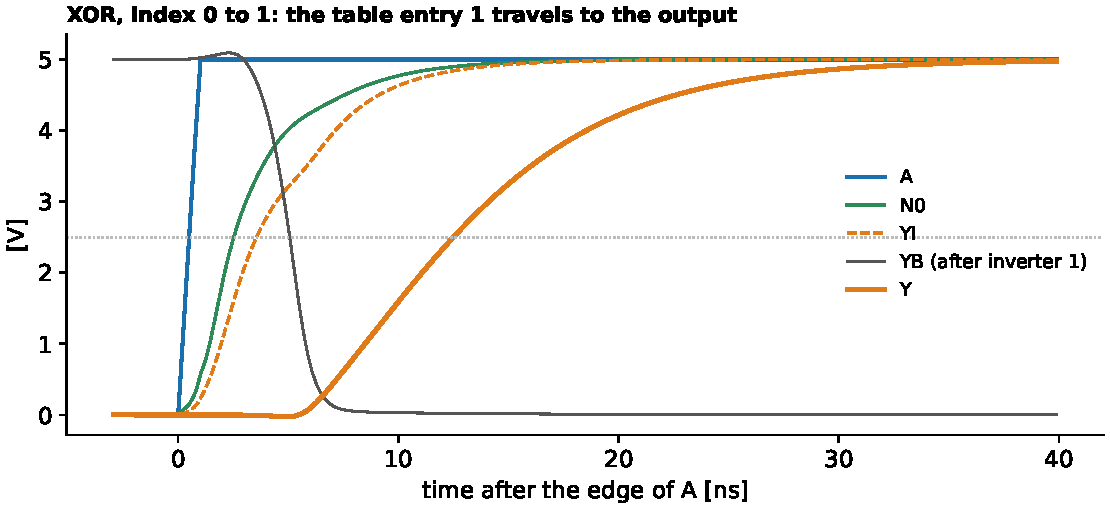
\includegraphics[width=\textwidth]{fig_delay.pdf}
\caption{One rising edge in the XOR window: $A$ rises at $t=0$ and
selects $T_1=1$. $N_0$ and $YI$ charge through the transmission
gates, the first inverter ($YB$) switches quickly, and the output $Y$
charges the \SI{10}{pF} load. The dotted line is half the supply,
where the delays are measured.}
\label{fig:delay}
\end{figure}

A LUT in a modern FPGA switches in tens of picoseconds, not
nanoseconds. The difference is entirely in the numbers: transistors a
thousand times smaller, capacitances a thousand times smaller, and no
\SI{10}{pF} load, since the LUT drives only the next multiplexer. The
structure is the same.

\subsection{When both inputs change at once}
\label{sec:glitch}

The Gray-code stimulus changes one input at a time. What happens when
two change at once? Consider XOR and the change from index~1 ($A=1$,
$B=0$) to index~2 ($A=0$, $B=1$). Both $T_1$ and $T_2$ are~1, so the
output should stay at~1 throughout. But the tree is a path, and the
path changes: before, the output was connected to $T_1$ through
\texttt{mux\_n0} and the lower input of \texttt{mux\_y}; after, it is
connected to $T_2$ through \texttt{mux\_n1} and the upper input. During
the change, $A$ switches the first level while $B$ switches the second,
and for a moment the output may be connected to $T_0$ or $T_3$, both
of which are~0, or to a first-level node that has not yet charged.

The simulation tests this in a second, short run
(Figure~\ref{fig:glitch}): both inputs change within \SI{1}{ns}, four
times, with XOR and then XNOR configured so that the old and the new
table entry are both~1. The internal node $YI$ dips at every change,
down to \SI{3.14}{V} in the worst case. The output $Y$ does not move:
its lowest value is \SI{5.00}{V}. The dip of $YI$ lasts a few
nanoseconds, shorter than the first inverter and the loaded output can
follow, and it does not reach the switching threshold of \SI{2.24}{V}.

\begin{figure}[H]
\centering
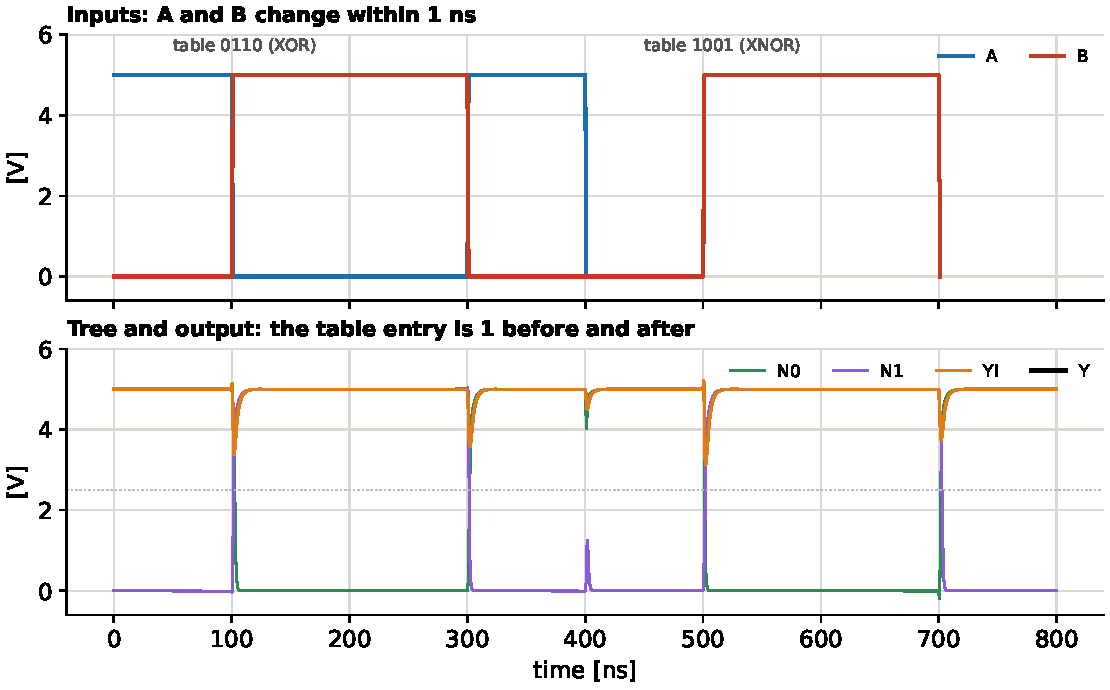
\includegraphics[width=\textwidth]{fig_glitch.pdf}
\caption{The glitch experiment. Both inputs change within \SI{1}{ns}
at \SIlist{100;300;500;700}{ns}; the table is XOR for the first
\SI{400}{ns} and XNOR afterwards, so that the selected bit is~1 before
and after every change. The tree output $YI$ dips at every change, to
\SI{3.14}{V} at worst; the buffered output $Y$ stays at \SI{5}{V}.}
\label{fig:glitch}
\end{figure}

This is a property of this circuit with these transistors and this
load, not of look-up tables in general. A faster LUT with a lighter
load, or a dip that went below $V_M$, would show a pulse at the output.
Such pulses are called glitches, and they are the reason that logic
built from LUTs is almost always synchronous: outputs are sampled by
registers at clock edges, when the trees have settled, and what they
do in between is allowed to be ugly. The LUT itself makes no promise
about the time between two valid states; the promise is made by the
clock.

\begin{merke}
The simulated LUT computes all 16 functions, 64 of 64 entries, with
full levels at every node and no current at rest. Delays of
\SIrange{8}{12}{ns} are set by the \SI{10}{pF} load and the \SI{4}{mA}
of the output PMOS; the input of the last tree level is the fastest.
When both inputs change at once, the tree output dips but the buffered
output does not: here. In general, a LUT's output is only guaranteed
once the tree has settled.
\end{merke}

% ============================================================
\section{What the model leaves out}
\label{sec:limits}
% ============================================================

Every number in this text is a property of the level-1 model with the
parameters of Section~\ref{sec:switch}. It is worth listing what that
model does not contain, so that the numbers are not mistaken for
properties of silicon.

\begin{itemize}
    \item \textbf{The transistors are generic.} Threshold \SI{1}{V},
          channel \SI{10}{\micro m} by \SI{10}{\micro m}, junction
          capacitance \SI{0.5}{pF}: these describe neither a discrete
          part nor an FPGA process. The level-1 model has no velocity
          saturation, no subthreshold current, no gate leakage. The
          \SI{0.015}{\micro A} at rest is the model's leakage, not a
          chip's.
    \item \textbf{The configuration is ideal.} Voltage sources have no
          output resistance and cannot be disturbed. Memory cells can,
          and a real LUT is sized so that reading a cell through the
          tree never flips it.
    \item \textbf{No layout.} Wiring capacitance and resistance are
          absent. There is a single load of \SI{10}{pF} at the output
          and nothing else.
    \item \textbf{Four-terminal transistors.} The bulk of every NMOS is
          at ground and of every PMOS at the supply, as on a chip. A
          discrete MOSFET has bulk and source tied together inside the
          package, and its body diode would conduct in a transmission
          gate whenever the drain is below the source. A breadboard
          version of this circuit therefore needs transistor arrays
          with a separate bulk pin, such as the CD4007.
\end{itemize}

None of these change the structure. They change the delays, the
current, and the margin against glitches, which is what a process
engineer would tune.

% ============================================================
\section{Summary}
\label{sec:summary}
% ============================================================

The common thread once more, in six steps:

\begin{enumerate}
    \item \textbf{A function is its truth table} (Boole 1854, Shannon
          1938). A function of $k$ inputs is $2^k$ bits; there are
          $2^{2^k}$ of them, 16 for $k=2$.
    \item \textbf{Store and select} (Shannon's expansion). A circuit
          that stores the $2^k$ bits and selects one with its inputs
          realises every function. Expanding $f$ one variable at a
          time, $f(A,B)=\ovl B\,f(A,0)+B\,f(A,1)$, yields a tree of
          2:1 multiplexers with the stored bits as leaves:
          $Y=T_{2B+A}$.
    \item \textbf{A switch is a transistor, but one is not enough}
          (Shichman--Hodges 1968). An NMOS passes a~1 only to
          $\VDD-\VT(V)$, \SI{3.51}{V} with the body effect; an NMOS
          and a PMOS in parallel, the transmission gate, pass both
          levels in full.
    \item \textbf{Inverters restore and drive} (Wanlass 1963). A CMOS
          inverter draws no current at rest and switches at
          $V_M=\SI{2.24}{V}$; two in series restore the level and
          polarity of the tree output and drive the load.
    \item \textbf{Twenty transistors and four bits.} Six transmission
          gates, two inverters for the complements, two for the
          buffer. The four bits are the configuration; here voltage
          sources, in an FPGA memory cells (Carter 1986, Freeman 1989).
    \item \textbf{The simulation confirms it} (Nagel 1973). All 16
          functions, 64 of 64 entries, delays of \SIrange{8}{12}{ns}
          into \SI{10}{pF}, the last tree level fastest, and a tree
          output that dips without the buffered output following.
\end{enumerate}

A word on size. This text has built a LUT with two inputs. The logic
element of a real FPGA has more: four inputs in the XC4000 family and
its contemporaries, the LUT4, and six inputs in current devices, the
LUT6 of the Xilinx 7~series and its successors~\cite{Xilinx4000,
Xilinx7}. There is no functional difference between these and the LUT2
of this text. A LUT4 stores $2^4=16$ bits and selects one of them with
a tree of four levels and 15 multiplexers; a LUT6 stores $2^6=64$ bits
behind six levels and 63 multiplexers. Shannon's expansion, the
transmission gate, the restoring buffer and the configuration by
stored bits are all the same; what grows is the number of leaves, the
depth of the tree, and with it the delay and the care needed against
glitches. A LUT6 drawn as a schematic would have 63 switch sheets and
would not fit on a page, and its simulation would have to step through
$2^{64}$ functions to be as complete as the one here. For readability
this text uses the LUT2, which is the smallest look-up table in which
the tree has two levels, so that the difference between a fast and a
slow input exists and can be measured. Everything said about it
applies, one level at a time, to the larger ones.

% ============================================================
\begin{thebibliography}{99}
% ============================================================

\bibitem{Boole1854} G.~Boole,
\emph{An Investigation of the Laws of Thought, on Which are Founded the
Mathematical Theories of Logic and Probabilities},
Walton and Maberly, London (1854).

\bibitem{Shannon1938} C.\,E.~Shannon,
\emph{A Symbolic Analysis of Relay and Switching Circuits},
Transactions of the American Institute of Electrical Engineers
\textbf{57}(12), 713--723 (1938).

\bibitem{Shannon1949} C.\,E.~Shannon,
\emph{The Synthesis of Two-Terminal Switching Circuits},
Bell System Technical Journal \textbf{28}(1), 59--98 (1949).

\bibitem{Lilienfeld1930} J.\,E.~Lilienfeld,
\emph{Method and Apparatus for Controlling Electric Currents},
U.S. Patent 1,745,175, filed 1926, issued 1930.

\bibitem{Kahng1960} D.~Kahng, M.\,M.~Atalla,
\emph{Silicon-Silicon Dioxide Field Induced Surface Devices},
IRE Solid-State Device Research Conference, Pittsburgh (1960).

\bibitem{Wanlass1963} F.\,M.~Wanlass, C.\,T.~Sah,
\emph{Nanowatt Logic Using Field-Effect Metal-Oxide Semiconductor
Triodes},
IEEE International Solid-State Circuits Conference, Digest of
Technical Papers, 32--33 (1963).

\bibitem{Shichman1968} H.~Shichman, D.\,A.~Hodges,
\emph{Modeling and Simulation of Insulated-Gate Field-Effect
Transistor Switching Circuits},
IEEE Journal of Solid-State Circuits \textbf{3}(3), 285--289 (1968).

\bibitem{Nagel1973} L.\,W.~Nagel, D.\,O.~Pederson,
\emph{SPICE (Simulation Program with Integrated Circuit Emphasis)},
Memorandum ERL-M382, Electronics Research Laboratory, University of
California, Berkeley (1973).

\bibitem{Gray1953} F.~Gray,
\emph{Pulse Code Communication},
U.S. Patent 2,632,058, filed 1947, issued 1953.

\bibitem{Carter1986} W.~Carter, K.~Duong, R.\,H.~Freeman, H.~Hsieh,
J.\,Y.~Ja, J.\,E.~Mahoney, L.\,T.~Ngo, S.\,L.~Sze,
\emph{A User Programmable Reconfigurable Logic Array},
Proceedings of the IEEE Custom Integrated Circuits Conference,
233--235 (1986).

\bibitem{Freeman1989} R.\,H.~Freeman,
\emph{Configurable Electrical Circuit Having Configurable Logic
Elements and Configurable Interconnects},
U.S. Patent 4,870,302, filed 1988, issued 1989.

\bibitem{Rose1990} J.~Rose, R.\,J.~Francis, D.~Lewis, P.~Chow,
\emph{Architecture of Field-Programmable Gate Arrays: The Effect of
Logic Block Functionality on Area Efficiency},
IEEE Journal of Solid-State Circuits \textbf{25}(5), 1217--1225 (1990).

\bibitem{Ahmed2004} E.~Ahmed, J.~Rose,
\emph{The Effect of LUT and Cluster Size on Deep-Submicron FPGA
Performance and Density},
IEEE Transactions on Very Large Scale Integration (VLSI) Systems
\textbf{12}(3), 288--298 (2004).

\bibitem{Xilinx4000} Xilinx, Inc.,
\emph{XC4000E and XC4000X Series Field Programmable Gate Arrays},
Product Specification DS009, Version 1.6 (1999).

\bibitem{Xilinx7} Xilinx, Inc.,
\emph{7 Series FPGAs Configurable Logic Block},
User Guide UG474, Version 1.8 (2016).

\bibitem{IEEE1364} IEEE,
\emph{IEEE Standard for Verilog Hardware Description Language},
IEEE Std 1364-2005, Section 18: Value change dump (VCD) files (2006).

\bibitem{SKiDL} D.~Vandenbout,
\emph{SKiDL: A Python package for describing electronic circuits},
\url{https://devbisme.github.io/skidl/}.

\bibitem{ngspice} H.~Vogt et al.,
\emph{Ngspice, the open source SPICE circuit simulator},
\url{https://ngspice.sourceforge.io/}.

\bibitem{Weste2011} N.\,H.\,E.~Weste, D.\,M.~Harris,
\emph{CMOS VLSI Design: A Circuits and Systems Perspective},
4th edition, Addison-Wesley (2011). Chapters 2 (MOS transistor
theory) and 9 (combinational circuit design, transmission gates).

\end{thebibliography}

\end{document}
